\chapter{TiDAL: Visualizing Gene Regulatory Networks}
\label{chap:tidal}

\section{Purpose}

A software library is only as useful if it can help produce better software applications.
Thus, the purpose of this chapter is to explain the implementation of a Graphene application in visualizing the output of the bioinformatics tool, TiDAL (Time-Dependent Activity Linker).
This chapter is relevant for providing evidence of the utility of Graphene in producing interactive graphics for browser-based scientific tools.
The flexibility and customizability of Graphene is demonstrated, which will help support its scientific merit.

\section{Motivation}
\subsection{Pathogenic infections involve temporal regulatory cascades}
\subsection{High throughput data combined with computational methods may be used to infer regulatory transcription networks}

\begin{figure}
  \centering
  \includegraphics[width=\textwidth,page=17,trim=0.37cm .65cm 0.37cm 0.3cm, clip=true]{images/Figures.pdf}
  \caption{TiDAL interface.}
  \label{Figure:tidal-landing}
\end{figure}

\begin{figure}
  \centering
  \begin{subfigure}[t]{0.3\textwidth}
    \includegraphics[width=\textwidth,page=18,trim=8.5cm 0cm 9cm 0cm, clip=true]{images/Figures.pdf}
    \caption{Heat map visualization of TiDAL output.
      The color scale correlates with upregulation of genes associated with transcription factor families (vertical axis) at time (horizontal axis).
    }
    \label{Figure:tidal-output-heatmap}
  \end{subfigure}
  \begin{subfigure}[t]{.66\textwidth}
    \includegraphics[width=\textwidth,page=19]{images/Figures.pdf}
    \caption{Table view of TiDAL output.
      Similar to the heatmap representation, the table provides all numerical data points generated by TiDAL in connecting transcription factor activity over time.
    }
    \label{Figure:tidal-output-table}
  \end{subfigure}
  \begin{subfigure}[b]{\textwidth}
    \includegraphics[width=\textwidth,page=20,trim=0.37cm 0.65cm 0.37cm 0.3cm, clip=true]{images/Figures.pdf}
    \caption{
      Graphene Network diagram of TiDAL output produced by Graphene.
      Transcription factors are represented as nodes and grouped by time activated.
      Edges indicate regulation between transcription factors.
      Red color edges indicate downstream regulation and green edges indicate upstream regulation.
      Upon  mouse hover over a node, its connect neighbors will be highlighted.
    }
    \label{Figure:tidal-output-graphene}
  \end{subfigure}
  \caption{Visualizations of TiDAL output.}
  \label{Figure:tidal-output}
\end{figure}

\autocite{zaslavsky2013reconstruction}


\subsection{Temporal regulatory cascades are high dimensional and benefit from visualization}


\section{Solution}
\subsection{Native HTML5 visualizations of TIDAL output}
\subsection{Layout style encoding to visualize high dimensional data}
\subsection{User interaction for network exploration}
Hovering

\section{Implementation}
\subsection{Graphene based web component}
\subsection{Data and layout controllers}
\subsection{Event handling}

\section{Future Directions}
